\section{Elementos regulatórios e Fatores de transcrição}

   \frame{\justifying
    \frametitle{Região reguladora}
      \begin{itemize}            
        \item Cada gene tem uma região regulatória, geralmente de 100-1000 pares de bases acima do local de início da transcrição.
		\item Dentro dela estão os elementos regulatórios.
	  \end{itemize}
	}
	
   \frame{\justifying
    \frametitle{Elementos regulatórios}
       \begin{itemize}            
        	\item	São pequenas sequências de DNA localizadas a uma distância aproximada de -50 pares de base do local de início da transcrição na região promotora de um gene (figuras \ref{fig:promotores_noDNA} e \ref{fig:localizacao_TFBS}).

			\item O tamanho aproximado dos elementos regulatórios varia entre 5 a 20 nucleotídeos.

			\item Cada elemento regulatório é específico a um fator de transcrição.
	   \end{itemize}
   }
   
\frame{
     \frametitle{Elementos regulatórios}
\begin{figure}[htb!]
    \centering
    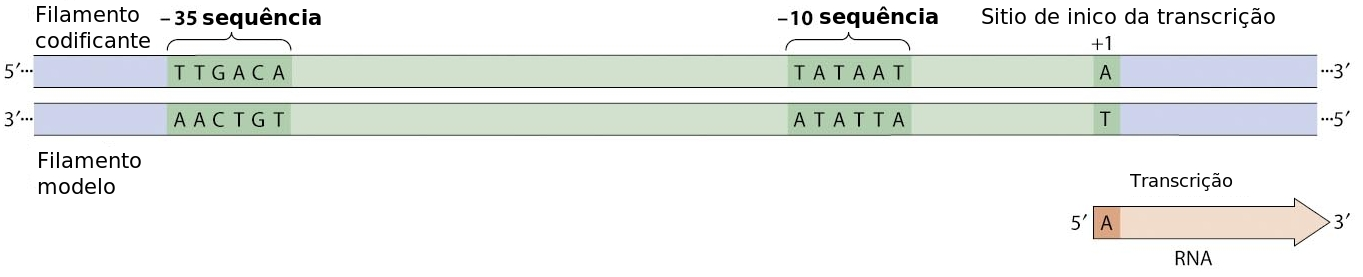
\includegraphics[scale=0.5]{./imagens/promotores_noDNA.jpg}
    \caption{Região promotora e as sequências consenso}
    \label{fig:promotores_noDNA}
\end{figure}
}

\frame{
     \frametitle{Elementos regulatórios}
    \begin{figure}[htb!]
    \centering
    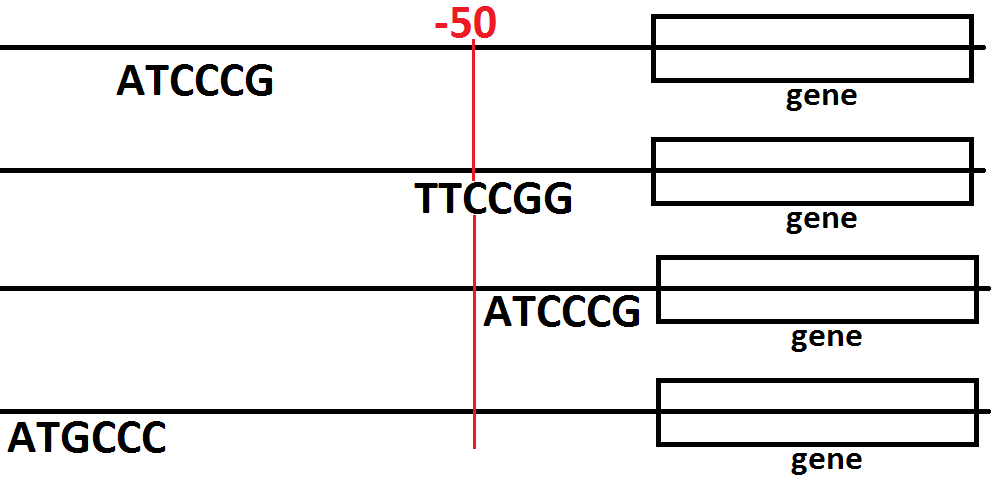
\includegraphics[scale=0.4]{./imagens/localizacao_TFBS.png}
    \caption{Localização aproximada dos elementos regulatórios}
    \label{fig:localizacao_TFBS}
    \end{figure}     
}

\frame{\justifying
     \frametitle{Fatores de Transcrição}
     Proteínas "especiais" chamadas de  \textbf{fatores de transcrição} (TF do inglês \textit{transcription factor binding site}) se ligam nos elementos regulatórios, contribuindo para o início da transcrição de um gene. Podem ser separados em fatores de transcrição gerais e específicos. (figuras \ref {fig:complexo_RNA-polimerase} e \ref{fig:TF_lingando_no_DNA}).

}

\frame{
     \frametitle{Fatores de Transcrição}
    \begin{figure}[htb!]
    \centering
    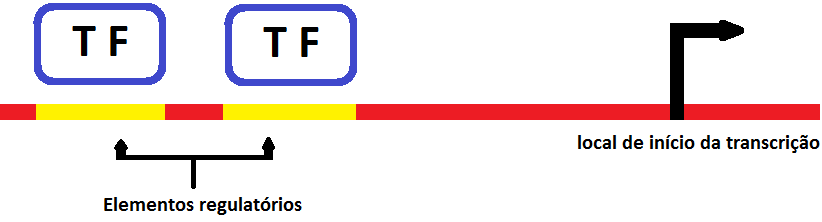
\includegraphics[scale=0.5]{./imagens/TF_lingando_no_DNA.png}
    \caption{Localização aproximada dos elementos regulatórios}
    \label{fig:TF_lingando_no_DNA}
    \end{figure}     
}

\frame{\justifying
	\frametitle{Funcionalidade na célula}
	Os elementos regulatórios juntamente com os fatores de transcrição funcionam como mecanismos de respostas a diversos estímulos, como:
	\begin{itemize}
		\item estímulos internos.
		\item estresses abióticos.
		\item estresses bióticos.				
	\end{itemize}
%    Estresses abióticos e bióticos influenciam negativamente na sobrevivência e na larga produção de grãos.
%	Existem elementos regulatórios que são ativados em resposta a estímulos como mudanças hormonais internamente em um organismo, ou externamente como: estresses abióticos que são causados por fatores não vivos como a alteração de temperatura e mudança climática, ou estresses bióticos causados por organismos vivos como bactérias, vírus, parasitas e insetos. Com a ativação do elemento regulatório ocorrera a expressão do gene, que o elemento regula, o gene será transcrito no RNA que posteriormente será traduzido, gerando proteínas para suprir as necessidades do organismo.
}

\frame{\justifying
	\frametitle{Funcionalidade na célula}
	Com a ativação de um elemento regulatório ocorre a expressão de um gene, que o elemento regula, o gene será transcrito no RNA que posteriormente será traduzido, gerando proteínas para suprir as necessidades do organismo.
}
